\chapter{Methods}
\label{chap:methods}



	\section{Basic fabrication elements}
    This section provides protocols for the basic fabrication building blocks put together in the construction of the different devices used in throughout this Ph.D work. Specific protocols for the assembly of such particular devices are further provided in the relevant chapters.

    \label{sec:methods:fabrication}
        \subsection{PDMS preparation}
        PDMS pre-polymers (Sylgard 184, Dow Corning) were mixed in the ratio 10:1 w/w base monomer to cross-linking catalyst, and de-gassed in a desiccator unit attached to a vacuum pump. The resulting viscous liquid was poured onto a mould or a substrate depending the application and de-gassed again if required. The PDMS was cured at 60-80\degree C for 2 hours or overnight.
        \label{sec:methods:PDMSMix}


        \subsection{SU-8 Embossing}
        To create microchannel moulds a thick film photoresist was required. SU-8 is known to allow features of high aspect ratio and vertical sidewall, both essential for microchannel fabrication. SU-8 film thickness is primarily determined by spin-coater speed and time, and by the ratio of solvent to epoxy in the photoresist. The higher the epoxy content, the more viscous it will be and more resist will remain after the spin-coating and heating steps described below.

        A 3 inch (\(76.2mm\)) silicon wafer was sonicated for 5 minutes in ethyl lactate and then rinsed in more of the same solvent. This process was repeated for acetone, methanol, and IPA. The wafer was dried under a nitrogen stream and dehydrated at 150\degree C for at least 30 minutes. SU-8 2050 was deposited onto the centre of the wafer and spun at 500rpm for 10 seconds to coat uniformly, followed by 30 seconds at 2000rpm to thin the photoresist to \(\approx 75\mu m\). The wafer was baked on a 65\degree C hotplate for 5 minutes followed by 95\degree C for 10 minutes, to remove all solvent from the photoresist.

        Photomasks of chrome on soda glass were designed using a CAD software (Autodesk Inventor Professional) and fabricated by JD Photo-tools Inc. Such designs of 2-port and 3-port channels are provided in figure \ref{fig:devices:basicDimensions}. After aligning the mask, the baked wafer was exposed to UV light at \(365nm\) and \(9\frac{mW}{cm^{2}}\) for 30 seconds. The exposed wafer was heated again for 5 minutes at 65\degree C and 10 minutes at 95\degree C, to cross-link the exposed regions of the SU-8. The wafer was immersed in ethyl lactate with mild agitation for 15 minutes, to strip off the unexposed SU-8 from the wafer. After rinsing with more ethyl lactate, the wafer and SU-8 features were heated to 150\degree C for 30 minutes and allowed to cool, in order to render the photoresist mechanically robust (hard bake). Measurement of the SU-8 features with a contact profilometer confirmed the height to be between \(60-100\mu m\).

        After the hard bake, the wafer was thermally glued (Epo-Tek) to a machined disk of aluminium \(76.2mm\) in diameter and \(2mm\) thick. This provided rigidity to the wafer, greatly reducing the possibility of it shattering if exposed to a flexing force during subsequent PDMS degassing and excising steps.
        The gluing process took 20 minutes on a 115\degree C hotplate. This temperature was chosen to ensure the SU-8 features were not reheated close to their glass transition point.
        \label{sec:methods:SU8}

        \subsection{Soft lithography}
        PDMS pre-polymers were mixed and degassed (section \ref{sec:methods:PDMSMix}). The pre-ploymer mix was then poured into a polystyrene petri dish containing a silicon wafer patterned with SU-8 (section \ref{sec:methods:SU8}).
        The PDMS was cured at 60\degree C for at least 2 hours or overnight at room temperature. After this time the PDMS was peeled off the mould and individual dies were separated with a scalpel. Fluid access ports were created with a \(0.5mm\) biopsy punch (ProSciTech), flushed with deionised water to remove debris, and nitrogen dried. The moulded face of the PDMS was cleaned \(3\times\) with scotch tape to remove remaining debris and dust. The process is illustrated in figure \ref{fig:methods:softLithography}.

        \begin{figure}[h]
            \centering
            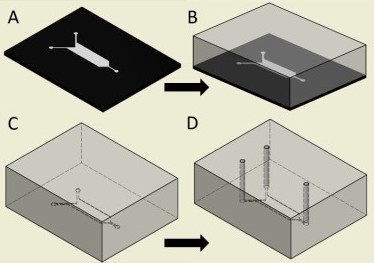
\includegraphics[scale=0.7]{chapter2/figures/softLithography/softLithographyProcess.jpg}
            \caption[Illustration of the soft lithography process]{\textbf{Illustration of the soft lithography process.} The SU-8 master mould (A) is covered with liquid PDMS (B). After curing at 60-80\degree C for 2 hours, the PDMS is excised with a scalpel and peeled from the mould (C). Access ports are cut with a biopsy punch (D). Figure was adapted from \cite{johnstoneThesis} with permission.}
            \label{fig:methods:softLithography}
        \end{figure}
        \label{sec:methods:softLitho}
        \subsection{Thin film spinning}
        To generate thin films of PMDS, the mixed pre-polymers were poured onto the central third of either a 3 inch (\(76.2mm\)) silicon wafer or a \(80\times 80 mm^{2}\) glass slide and processed on a spin-coater (SPS Europe Spin 150), with film thickness determined by spin RPM and time. The substrate with the pre-polymer film was then transferred to a hotplate at 100\degree C and baked for 5 minutes, to harden the PDMS film and heat the substrate. Next, we applied a grid of thick PDMS strips to the top of the thin film. Due to the high temperature of the substrate the PDMS strips did not spread and hardened immediately thus forming think tabs around rectangular PDMS sheets which were cut out and used as the microwell layer in specific device designs. The thick tabs were required because the thin film cannot be handled unsupported. After application of the strips the substrate was left at 100\degree C for at least 30 minutes. The glass slides were used as the substrate when the features in the PDMS sheet were manually excised because a printout of the geometry placed underneath for reference could be observed. This was the case for the devices used in chapter \ref{chap:microculturePulses}. We used 2 spin speeds with the glass slides, 700 and 1000 RPM, applied for 30 seconds. These speeds resulted in film thicknesses of \(118\pm 21\) or \(79\pm 9\mu m\), respectively (figure \ref{fig:methods:profiles}).
        \begin{figure}[h]
            \includegraphics[width=14cm]{chapter2/figures/profiles/spin_profiles.jpg}

            \caption[Profiling of PDMS thin film thicknesses]{\textbf{Profiles showing the thin film thickness obtained using the 2 spin speeds in use.} Measurements were made with a micro-tip profiler and show the step between a stretch of exposed substrate and the thin film. Solid lines show the mean across measured samples and shaded areas represent the standard deviation. Dashed lines show the mean of a step function fit which was applied to each of the measurements. Data is based on n=4 and 3 samples for 700 and 1000 RPM, respectively.}
            \label{fig:methods:profiles}
        \end{figure}
        Silicon wafers were used under a fabrication paradigm by which the liquid pre-polymer is poured onto an SU-8 mold and so the thin film is cured with the desired shapes already cut out of it. The SU-8 mold was pre-fabricated as in section \ref{sec:methods:SU8}. For this approach to be successful the thickness of the thin film needs to be smaller than the height of the SU-8 as otherwise the mold will only leave a dent in the film rather than completely punch out the desired shape. Achieving the required thickness required a spin speed of 2000 RPM for 30 seconds. An undesirable side effect of this approach was that the liquid pre-polymer rose to a higher level around the SU-8 features compared to the bulk thickness due to a meniscus effect (figure \ref{fig:methods:mwProfile}). This paradigm was used in section \ref{sec:devices:microcultures} which also shows an example design.

        \begin{figure}[h]
            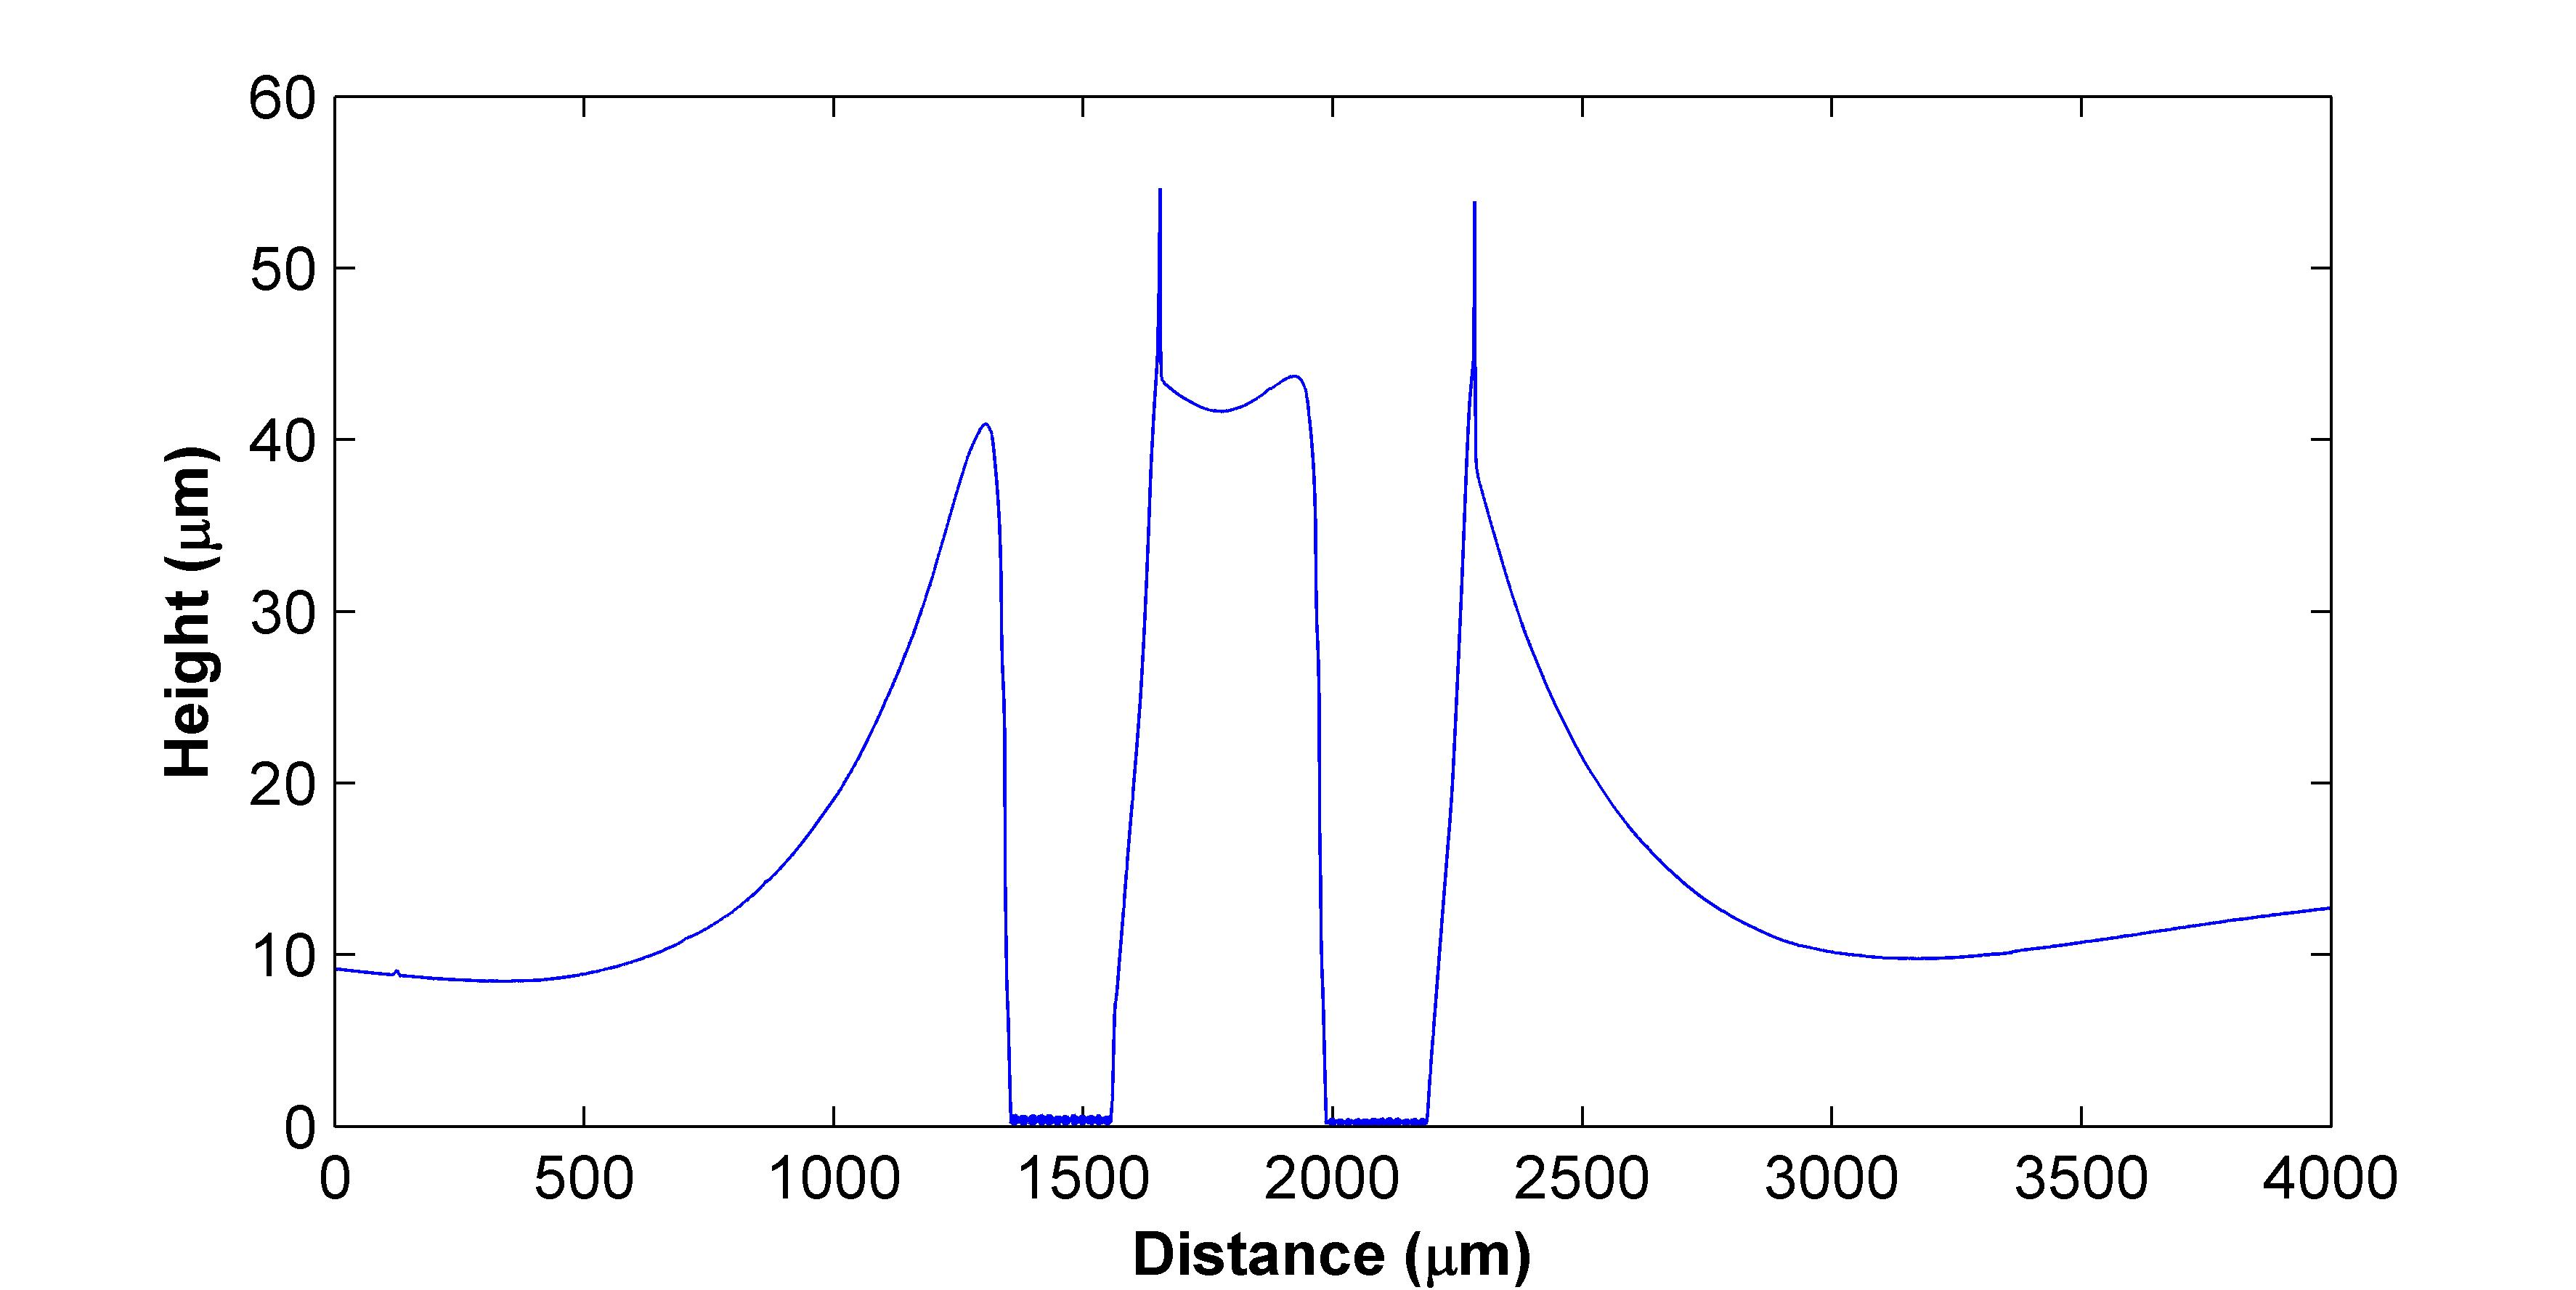
\includegraphics[width=14cm]{chapter2/figures/mw_profile/mw_profile.jpg}
            \label{fig:methods:mwProfile}
            \caption[Representative profile of a PDMS with microwells manufactured by spinning liquid pre-polymer on a SU-8 mold]{\textbf{PDMS sheets with microwells manufactured by pouring liquid pre-polymer on a SU-8 mold were characterized by a an elevated ridge around the cut out shapes.} The measurement was made with a micro-tip profiler on a PDMS sheet with a pair of \(300 \mu m\) microwells. The sharp peaks on the right edges of the microwells are an artefact resulting from the PDMS being dragged up by the profiler tip.}
        \end{figure}


        \subsection{PDMS extraction}
        PDMS extraction was required to avoid cytotoxicity associated with oligomer leaching in certain devices, namely the ones used in chapters \ref{chap:devicesAndFlow} and \ref{chap:microculturePulses}. The extraction protocol was based on \cite{millet2007microfluidic}. Engraved PDMS blocks or cut out thin films were transferred into a Duran bottle and subjected to the following solvent immersion steps (hours): Pentane (16, Sigma, 158941-2.5L), Pentane (8), Xylenes (1, Sigma, 247642-2.5L), Xylenes (16), Xylenes (8), IPA (1, Fischer Chemical, P/7507/PB17), IPA (16), IPA (8), DDW (8). After the solvent immersion the devices were placed in a 120\degree C oven for at least 56 hours. This was required to completely remove the solvent chemicals which are themselves very toxic.


    \section{Bonding techniques}
    \label{sec:methods:bonding}
    \subsection{Plasma bonding}
        Oxygen plasma activation creates hydroxyl (OH\textsuperscript{-}) groups on surfaces. Where silicon (Si) atoms are present as in glass and PDMS, the OH\textsuperscript{-} groups will covalently bind to them.

        PDMS surfaces were pre-cleaned \(3\times\) with scotch tape. Glass surfaces were pre-treated in the same way that they were prepared for surface chemistry (section \ref{sec:methods:surface}). The parts were placed in a plasma oven with the active surfaces facing up. The parts were oxygen (N\textsubscript{2} free) plasma-activated at \(50W\) and \(200 mTorr\) for 30 seconds. Activated parts were removed from the oven and bonded within 2 minutes, before the OH\textsuperscript{-} groups could be passivated by moisture content in the air. Where careful alignment between surfaces was needed, (two layer microwell devices, section \ref{sec:devices:microcultures}) a low magnification microscope (dissection-scope) was used. Bonded devices were finally transferred to a 120\degree C oven where they were kept for 2 hours to facilitate the covalent bonding and to render them sterile.

        \subsection{Double sided silicone tape}
        Silicone-based adhesive transfer tapes of thickness \(50\mu m\) or \(125\mu m\) (3M, 91022 or 96042, respectively) were used. The tapes are provided with a white polyethylene terephthalate (PET) primary release liner, and were backed onto an optically clear Polyester (PE) secondary release liner (also 3M). Geometries were designed using CAD software (Autodesk Inventor Professional) and exported in .dxf format to a plotter cutter (Silhouette Cameo, Graphtec) which excised them from the liner-tape-liner stack. Devices were assembled starting with a bulk PDMS layer. PDMS was mixed, cast and cured as described previously (section \ref{sec:methods:softLitho}) in a petri dish with no feature mould so that a smooth flat surface was formed for the tape to adhere to. The secondary release layer was removed from the tape and the exposed silicon adhesive brought into contact with the PDMS. Flow connections were punched using a \(0.5mm\) biopsy punch (ProSciTech) and cleaned of debris by pushing DDW through them. The primary release liner was then removed and the second adhesive surface brought into contact with either a glass coverslip or an MEA. Initial contact was performed at room temperature.

        \begin{figure}[h]
            \centering
            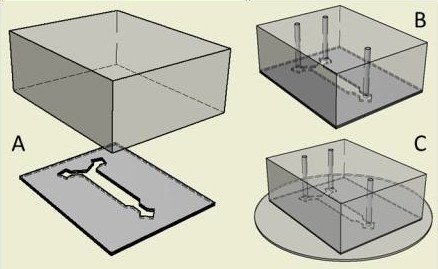
\includegraphics[scale=0.7]{chapter2/figures/tapeBonding/tapeBonding.jpg}
            \caption[Illustration of tape-based device fabrication process]{\textbf{Illustration of tape-based device fabrication process.} The secondary liner is removed and the tape flipped over to adhere to the PDMS (A). Once adhered, access ports are cut with a biopsy punch (B), before the primary liner is removed and the device attached to glass (C). Figure was adapted from \cite{johnstoneThesis} with permission.}
            \label{fig:methods:tapeBonding}
        \end{figure}
        \label{sec:methods:tape}

        \subsection{Pre-polymer bonding}
        The \(19mm\) coverslips were cleaned as in section \ref{sec:methods:surface} and the PDMS channels were produced as in section \ref{sec:methods:softLitho}. A \(22mm\) diameter coverslip was placed on the spin-coater. A few drops of PDMS curing pre-polymer were pipetted onto the glass and the coverslip was then spun at 2000 RPM for 30 seconds, leaving a \(20\mu m\) layer of pre-polymer. With the \(22mm\) coverslip vacuum clamped in place, the PDMS channel was brought into contact with the pre-polymer layer for a few seconds and then lifted off. This coated the base surface of the PDMS with catalyst while leaving the channel unaffected. The PDMS was then placed in contact with the \(19mm\) glass coverslip. The device was finally placed in a 120\degree C for 2 hours for curing and sterilization.


        \begin{figure}[h]
            \centering
            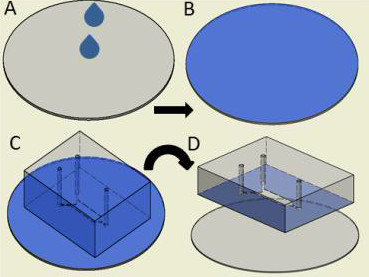
\includegraphics[scale=0.7]{chapter2/figures/glueBonding/glueBonding.jpg}
            \caption[Illustration of the pre-polymer bonding process]{\textbf{Illustration of the pre-polymer bonding process.}  Catalyst is pipetted onto a \(22mm\) coverslip (A) and spun to a uniform thickness (B). PDMS channel is stamped on the catalyst (C) and transferred to a \(19mm\) coverslip (D) before thermal curing of the catalyst. Figure was adapted from \cite{johnstoneThesis} with permission.}
            \label{fig:methods:glueBonding}
        \end{figure}


    \section{Surface coating}
    \label{sec:methods:surface}
        \subsection{PLL coating}
        To coat open surfaces (e.g., MEAs in chapter \ref{chap:activity}) they were incubated (37\degree C, 90\% humidity) overnight with 0.5 ml drop of 0.01\% PLL solution (Sigma, P4707-50ML) in the centre. The next morning, the PLL was removed and the surfaces were washed with DDW \(2-3\times\). In each washing step the surfaces were left immersed in the DDW for a few minutes to allow dissolution of free PLL oligomers. Finally, the surfaces were left uncovered in the sterile hood for at least 2 hours to dry. In cases where `surface-then-bond' device assembly approach was used (used in section \ref{sec:devices:bonding}), a flow layer excised from a double sided silicone tape and already joined to a PDMS bulk (section \ref{sec:methods:tape}) was glued to the surface at this point.

        To coat the internal surface of a device after it had been assembled, i.e., `bond-then-surface' (used throughout most of section \ref{sec:devices:protocolDev}), the assembled devices were flushed with PLL by placing a \(200\mu l\) drop on top and pulling through with a \(1ml\) plastic syringe. The devices were incubated as above overnight in a \(90mm\) petri dish with an accompanying smaller dish containing DDW to reduce evaporation. The next morning, all PLL was removed by pulling with a \(1ml\) syringe and devices were flushed twice with growth media (see section \ref{sec:methods:culture}).

         Both surface-then-bond and bond-then surface devices were finally immersed in \(2.5-3 ml\) of growth media. The immersion ideally occurred the night before the cell seeding because it induced a slow bubble formation within the channel due to air escaping the PDMS as it became wetted. Thus further and final flushing was performed the next day to remove the trapped air bubbles.

        \subsection{PEI coating}
        Following chapter \ref{chap:devicesAndFlow} we switched to using exclusively PEI for surface coating as it is known to produce better adhesion as compared to PLL on some surfaces \cite{wiertz2010regulation}. Indeed we found that using PEI gave rise to more consistent preparations. PEI required adherence to a strict protocol to make sure that no soluble monomers, which are very toxic, are present.

        To prepare the coating solution, 50\% PEI (Sigma, P3143-100ML) was diluted \(500\times\) in DDW (sonication was required for complete dissolution) and sterile filtered. To coat open surfaces a \(0.5ml\) drop of the coating solution was pipetted on the surface center and left in room temperature for 2 hours. The surfaces were then washed with DDW thrice whereby in the final washing step they were immersed in DDW for 2 hours. Finally they were left in the hood to dry for at least a few hours, typically overnight. At this point, tape and PDMS layers were joined to the surface to complete the assembly of the device. In the case of MEAs a glass cylinder was glued to hold the immersion media (see image in figure \ref{fig:pulses:circularIllustration}). The final pre-seeding immersion was performed as described above for the PLL but with \(4ml\) of media to ensure enough supply for `self media' flow experiments (see section \ref{sec:crossFlow:intro}).

 \section{Seeding and maintaining of Neuronal cultures}
 We used growth media based on Neurobasal (Invitrogen, 21103-049) supplemented with B27 (Invitrogen, 17504-044) and and \(0.5mM\) L-Glutamine  (Sigma, G7513). Harvesting of primary hippocampal and cortical cells seeding solutions was as follows: the entire cortices of E-18 pregnant rat embryos were removed. Cortices were then subjected to further dissection for precise removal of the meninges and excision of the hippocampi. Hippocampi and 2-3 cortices were then each placed in a dish with \(2ml\) Hank's solution with 0.1\% trypsin and 0.005\% DNAse (Sigma, D5025-15KU) for 20 minutes following which 0.05\% trypsin inhibitor (Sigma, T9003) was added to de-activate the trypsin. The tissue was then transferred to a falcon tube, washed once and suspended in \(1.5ml\) growth media with 0.005\% DNAse. Next, the tissue was triturated with a flame polished glass pasteur until the cells were fully in suspension. The cells were then centrifuged and re-suspended again in \(1.5ml\) growth media. Finally, the cells were counted and diluted or concentrated as necessary (by centrifuging and re-suspending) to the final required seeding density.

 Open MEAs were seeded by placing a \(0.5ml\) drop of cortical seeding solution in the centre of the sample. The cells were allowed to settle for 30 minutes in the incubator, after which the media was topped up to \(1ml\). This is relevant to all the samples used in chapter \ref{chap:activity}.

 Devices were seeded by injecting \(1-3\mu l\) of hippocampal seeding solution into the outlet port using a gel-loading tip. In all microculture devices as well as devices used for flow with self media (see section \ref{sec:crossFlow:intro}) external support cultures were seeded as well. These comprised further cortical cells plated on the exposed coverslip or MEA surface around the PDMS device at a volume density of \(50-100 \frac{cells}{\mu l}\). In the case of microculture devices, a further flushing step was employed the following day to remove excess cells residing outside the microwell. The microculture devices in section \ref{sec:devices:microcultures}, where the surface outside the microwells was cell adhesive, required aggressive flushing which was performed by pulling media through with \(1ml\) syringe. This action selectively removed cells from the top of the PDMS sheet and not from the within the microwell by virtue of the shear protection that it confers. However, in some cases a noticeable amount of cells were removed also from the wells. In contrast, the microculture devices in chapter \ref{chap:microculturePulses}, where the surface outside the microwells was not cell adhesive, were conducive to gentle flushing which was performed by pushing \(20\mu l\) media through the channel using a syringe driver at a rate of \(50-100\frac{\mu l}{min}\). In this way, no cells were removed from the microwells.

 After plating, devices were placed in a humidified 5\% CO\textsubscript{2} incubator. Media in device preparations was changed by replacing approximately a third of the immersion media. Media change was normally performed twice a week. However, for samples in chapter \ref{chap:microculturePulses} the media was changed only 3 times to maximize its saturation with conditioning factors towards its subsequent use for self media flow.


         \label{sec:methods:culture}

\section{MEA recording and stimulation}
Multi electrode array recordings were performed with commercial MEAs (Multi Channel Systems, 60MEA200/30-Ti or 60HDMEA30/10iR-ITO). Electrical activity was recorded with a 60-channel USB amplifier system (USB-MEA60-Inv, Multi Channel Systems) fitted in the environmental chamber (37\degree C) and using MCRack recording software (Multi Channel Systems) with 2nd order Butterworth band pass filtering (\(200-3000Hz\)).

\label{sec:methods:MEARecording}

\subsection{Spike detection and noise removal}
Preliminary spike detection was performed in real time using MC Rack whereby only \(20 ms\) windows around threshold crossings were stored. These thresholds were channel specific and were typically automatically set to \(-5.5\) standard deviations of the channel baseline noise. This definition catered for most extracellular spike shapes where the peak deflection was negative. In the minority of cases, where most spikes in the channel had a positive peak deflection (sometimes termed inverted spikes) we set the threshold to \(+5.5\). A second filtering step utilized the wavelet packet decomposition method and software package from \cite{hulata2002method} to exclude noise. In essence this is based on a wavelet function optimized to best represent noise features and so spikes were further excluded by applying a second threshold to the correlation between the spike waveform and the noise wavelet. Examples of this procedure and the effect of the second threshold are provided in figure \ref{fig:methods:matchFilter}.

\begin{figure}[!htb]
\centering
\includegraphics[width=15cm]{chapter2/figures/matchFilter/matchFilterIllustration.jpg}
\caption[Examples of spike detection and shape based artefact removal]{\textbf{A two-step spike detection procedure is effective at excluding spike artefacts.} 3 example windows of filtered electrical data (band pass \(200-3000Hz\)). Initially spike times are determined by crossings of electrical threshold (marked by cyan lines). However, spike waveforms (marked by a color overlay in a \(2ms\) window around crossings) are further subjected to correlation with a wavelet function representative of noise. Thus a second threshold is applied to the correlation to exclude noise-resultant spike waveforms. Application of second threshold is exemplified using two values. Spikes marked by green overlay are ones accepted by both correlation thresholds and those marked in red are excluded by the higher threshold. The higher correlation threshold value (34) was the value used for spike detection throughout this work. The units for the second threshold are arbitrary (the value is derived from an un-normalized correlation function).}

\label{fig:methods:matchFilter}

\end{figure}

We found that the above shape based spike detection procedure was effective at removing some spike artefacts but in many cases they were erroneously retained. Most obvious were cases where, presumably due to external electromagnetic induction, such artefact spikes were elicited simultaneously across many channels, if not all. Such cross channel artefact spiking events were significantly more synchronized than even real neuronal bursts and so could be easily discerned simply by applying a threshold to the summated firing rate plot (where the former types of events were characterized by sharp peaks). Thus a final noise exclusion step was routinely employed where all spikes in a \(5ms\) window around such synchronized artefact spiking events were removed (figure \ref{fig:methods:syncArtefact}).

\begin{figure}[!htb]
\centering
\includegraphics[width=14cm]{chapter2/figures/syncArtefact/syncArtefact.jpg}
\caption[Example for synchrony based spike artefact removal]{\textbf{Synchronized spike artefacts events are easily discerned from actual biological bursting events via their increased synchronicity.} (A-B) A channel raster plot segment and its summation plot at \(1ms\) binning. (C) Filtered electrical data from one of the electrodes showing the detected spikes as red overlays. The rightmost detected spike is an artefact. (D-E) Same raster plot and summation as in A-B after removing the spikes associated with the artefact event. The event was detected by applying a threshold (in this case set to 10 spikes) to B and all spikes in a \(5ms\) window around the threshold crossing were excluded.}

\label{fig:methods:syncArtefact}

\end{figure}

\subsection{Electrical stimulation}
Individual stimulations consisted a rectangular and biphasic \(800 ms\)-long voltage pulses of \(300-900 mV\) were applied to the selected electrodes using either a 2-channel stimulus generator (STG 2002, Multi Channel Systems) or a data acquisition card capable of generating analogue voltage signals (DAQ, National Instruments, SCB-68A). The latter option was used for the plasticity protocol in section \ref{sec:activity:plasticityProtocol} where a complex stimulation sequence including both test pulses and tetanus was required. In this case, custom made Labview software was employed.

\label{sec:methods:stim}


\subsubsection{Automatic detection of responsive channels}
In some cases, the stimulation response data was presented in the form of a response chart which reflects the spatial arrangement of the recording channels and the of response in each is indicated via color coding. The response, in this case, is measured as the average number of spikes recorded in this channel at a time window \(10-210ms\) from the stimulation time (see examples in fig \ref{fig:activity:stimExample}). To make the charts clearer, we sought to exclude channels which were occasionally active during the above observation window by chance, due to ongoing spontaneous activity. Consequently, we employed a procedure where we collected the mean firing rates in the observations windows (i.e., \(10-210ms\) after the stimulation) for all stimulations as well as the mean firing rates in windows that are \(500ms\) distant from any stimulation and therefore represent the ongoing spontaneous activity. A t-test was employed between the above groups of measures and only channels showing significantly higher firing rate in the first window were kept and indicated in the chart. The significance threshold depended on the number of stimulations performed in the specific experiment and was therefore selected purely on the basis of obtaining visually pleasing results.


\subsection{Correlation maps}
To produce correlation maps, i.e., a correlation matrix, channel rasters at \(1ms\) binning were convolved with a gaussian kernel of width \(\sigma=100ms\). The correlation between pair of channels was simply defined as the Pearson correlation coefficient between the respective gaussian smoothed rasters. In some cases, a surrogate correlation map was computed based on the same data but where all the channel rasters were replaced by independent poisson processes with the same firing rate as in the respective channels (i.e., \(\lambda\) set to be the original channel firing rate). This procedure is illustrated in figure \ref{fig:methods:corrIllustration}.

\label{sec:methods:corrMaps}
\begin{figure}[!htb]
    \centering
    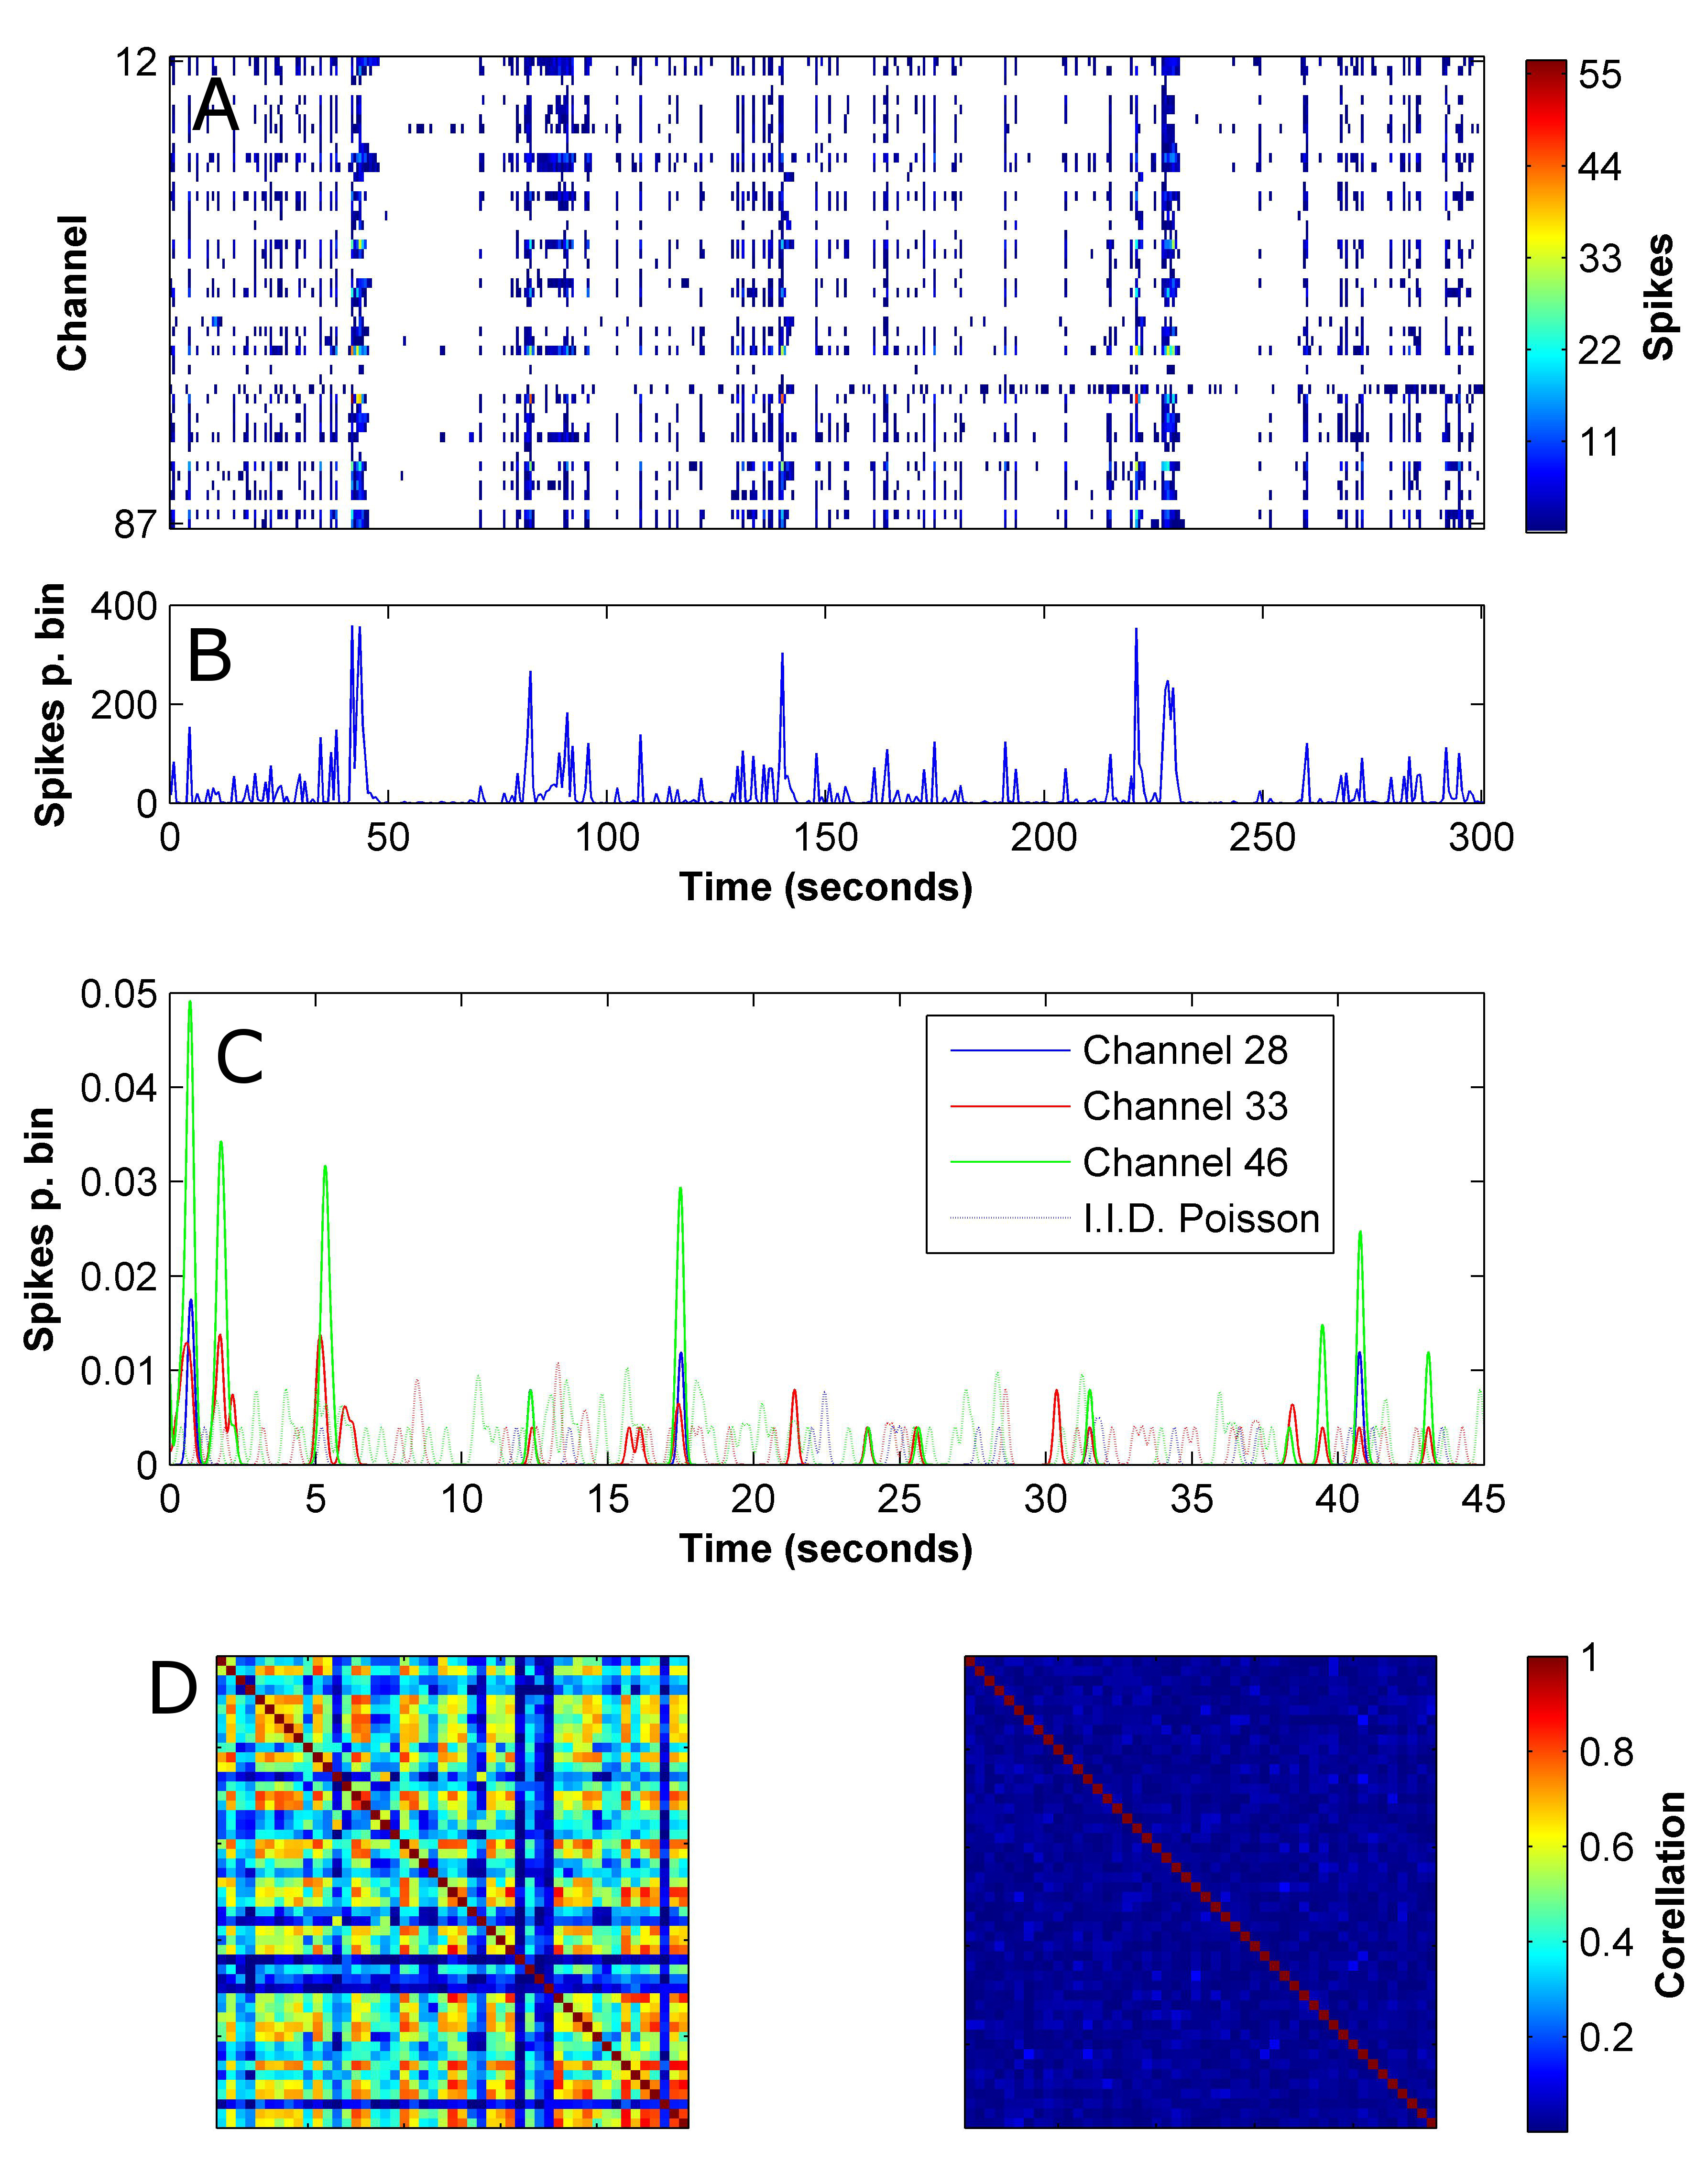
\includegraphics[width=14cm]{chapter2/figures/corrIllustration/corrIllustration.jpg}
    \caption[Computation of correlation maps]{\textbf{Comparison to surrogate maps based on independent poisson raster with firing rates as in the original data highlight the correlations in the data.} (A-B) Channel raster plots and their summation at \(0.6s\) binning. (C) Gaussian smoothed raster plot for 3 channels from the recording shown in A-B. Surrogate smoothed raster plots are shown for the same channels in dotted lines with same color coding. Evidently, the original data is significantly more correlated. (D) Correlation maps for original data (left) and surrogate (right).}
    \label{fig:methods:corrIllustration}
\end{figure}
\subsection{Burst detection}
Bursts are usually detected by applying a threshold to the firing rate plot. In contrast to previous attempts \cite{wagenaar2006extremely,chiappalone2005burst} where the threshold was somewhat arbitrary, we have devised a method to select an informed threshold value that would reflect whether the channels are synchronized or independent. To obtain such a threshold for a given recording we generated surrogate channel raster plots where the spike times were randomly drawn from a Poisson process with a rate parameter (\(\lambda\)) set to be the firing rate of the corresponding channel in the original data. These surrogate raster plots were summated, smoothed with a gaussian kernel with \(\sigma=70ms\) and the threshold was set to be 5 standard deviations above the mean of the resultant signal. Thus, all peaks above this threshold in the smoothed raster plot sum in the original data were defined to be bursts. Bursts that were closer than \(100ms\) were grouped into one whose time was taken to that of the highest peak.

The next stage of the analysis was to find burst limits (start and end). This process utilized two thresholds. One (firing rate threshold) was set, as before, to be 5 standard deviations over the mean of the surrogate smoothed raster plot sum curve. The second (derivative threshold) was set to be just the standard deviation of the derivative of the same surrogate curve. The start and end of a burst were defined as the closest points on the smoothed raster plot sum around the burst peak where the curve dips below the firing rate threshold, where the absolute value of the first derivative is below the derivative threshold and where the second derivative is positive. Since a relatively wide smoothing kernel was required which caused blurring of sharp event boundaries, we finally shifted the start and end points defined by the above criteria towards the peak, by half of the kernel width. The first threshold implements the original intuitive idea whereby the burst is a time window where the summated network activity is elevated as compared to what is anticipated by the surrogate raster plots. The second threshold can be thought of as applying the same intuitive idea but on the derivative. This extra threshold was required because when the boundaries were defined based only on the first one, they were sometimes so close that the final half kernel shifting caused the end time to be earlier than the start. The final threshold was required to make sure that points around troughs are detected and not around burst peaks. Examples of output from this procedure are shown in figure \ref{fig:methods:burstDet}.


\label{sec:methods:burstDetection}
\begin{figure}[!htb]
            \centering
            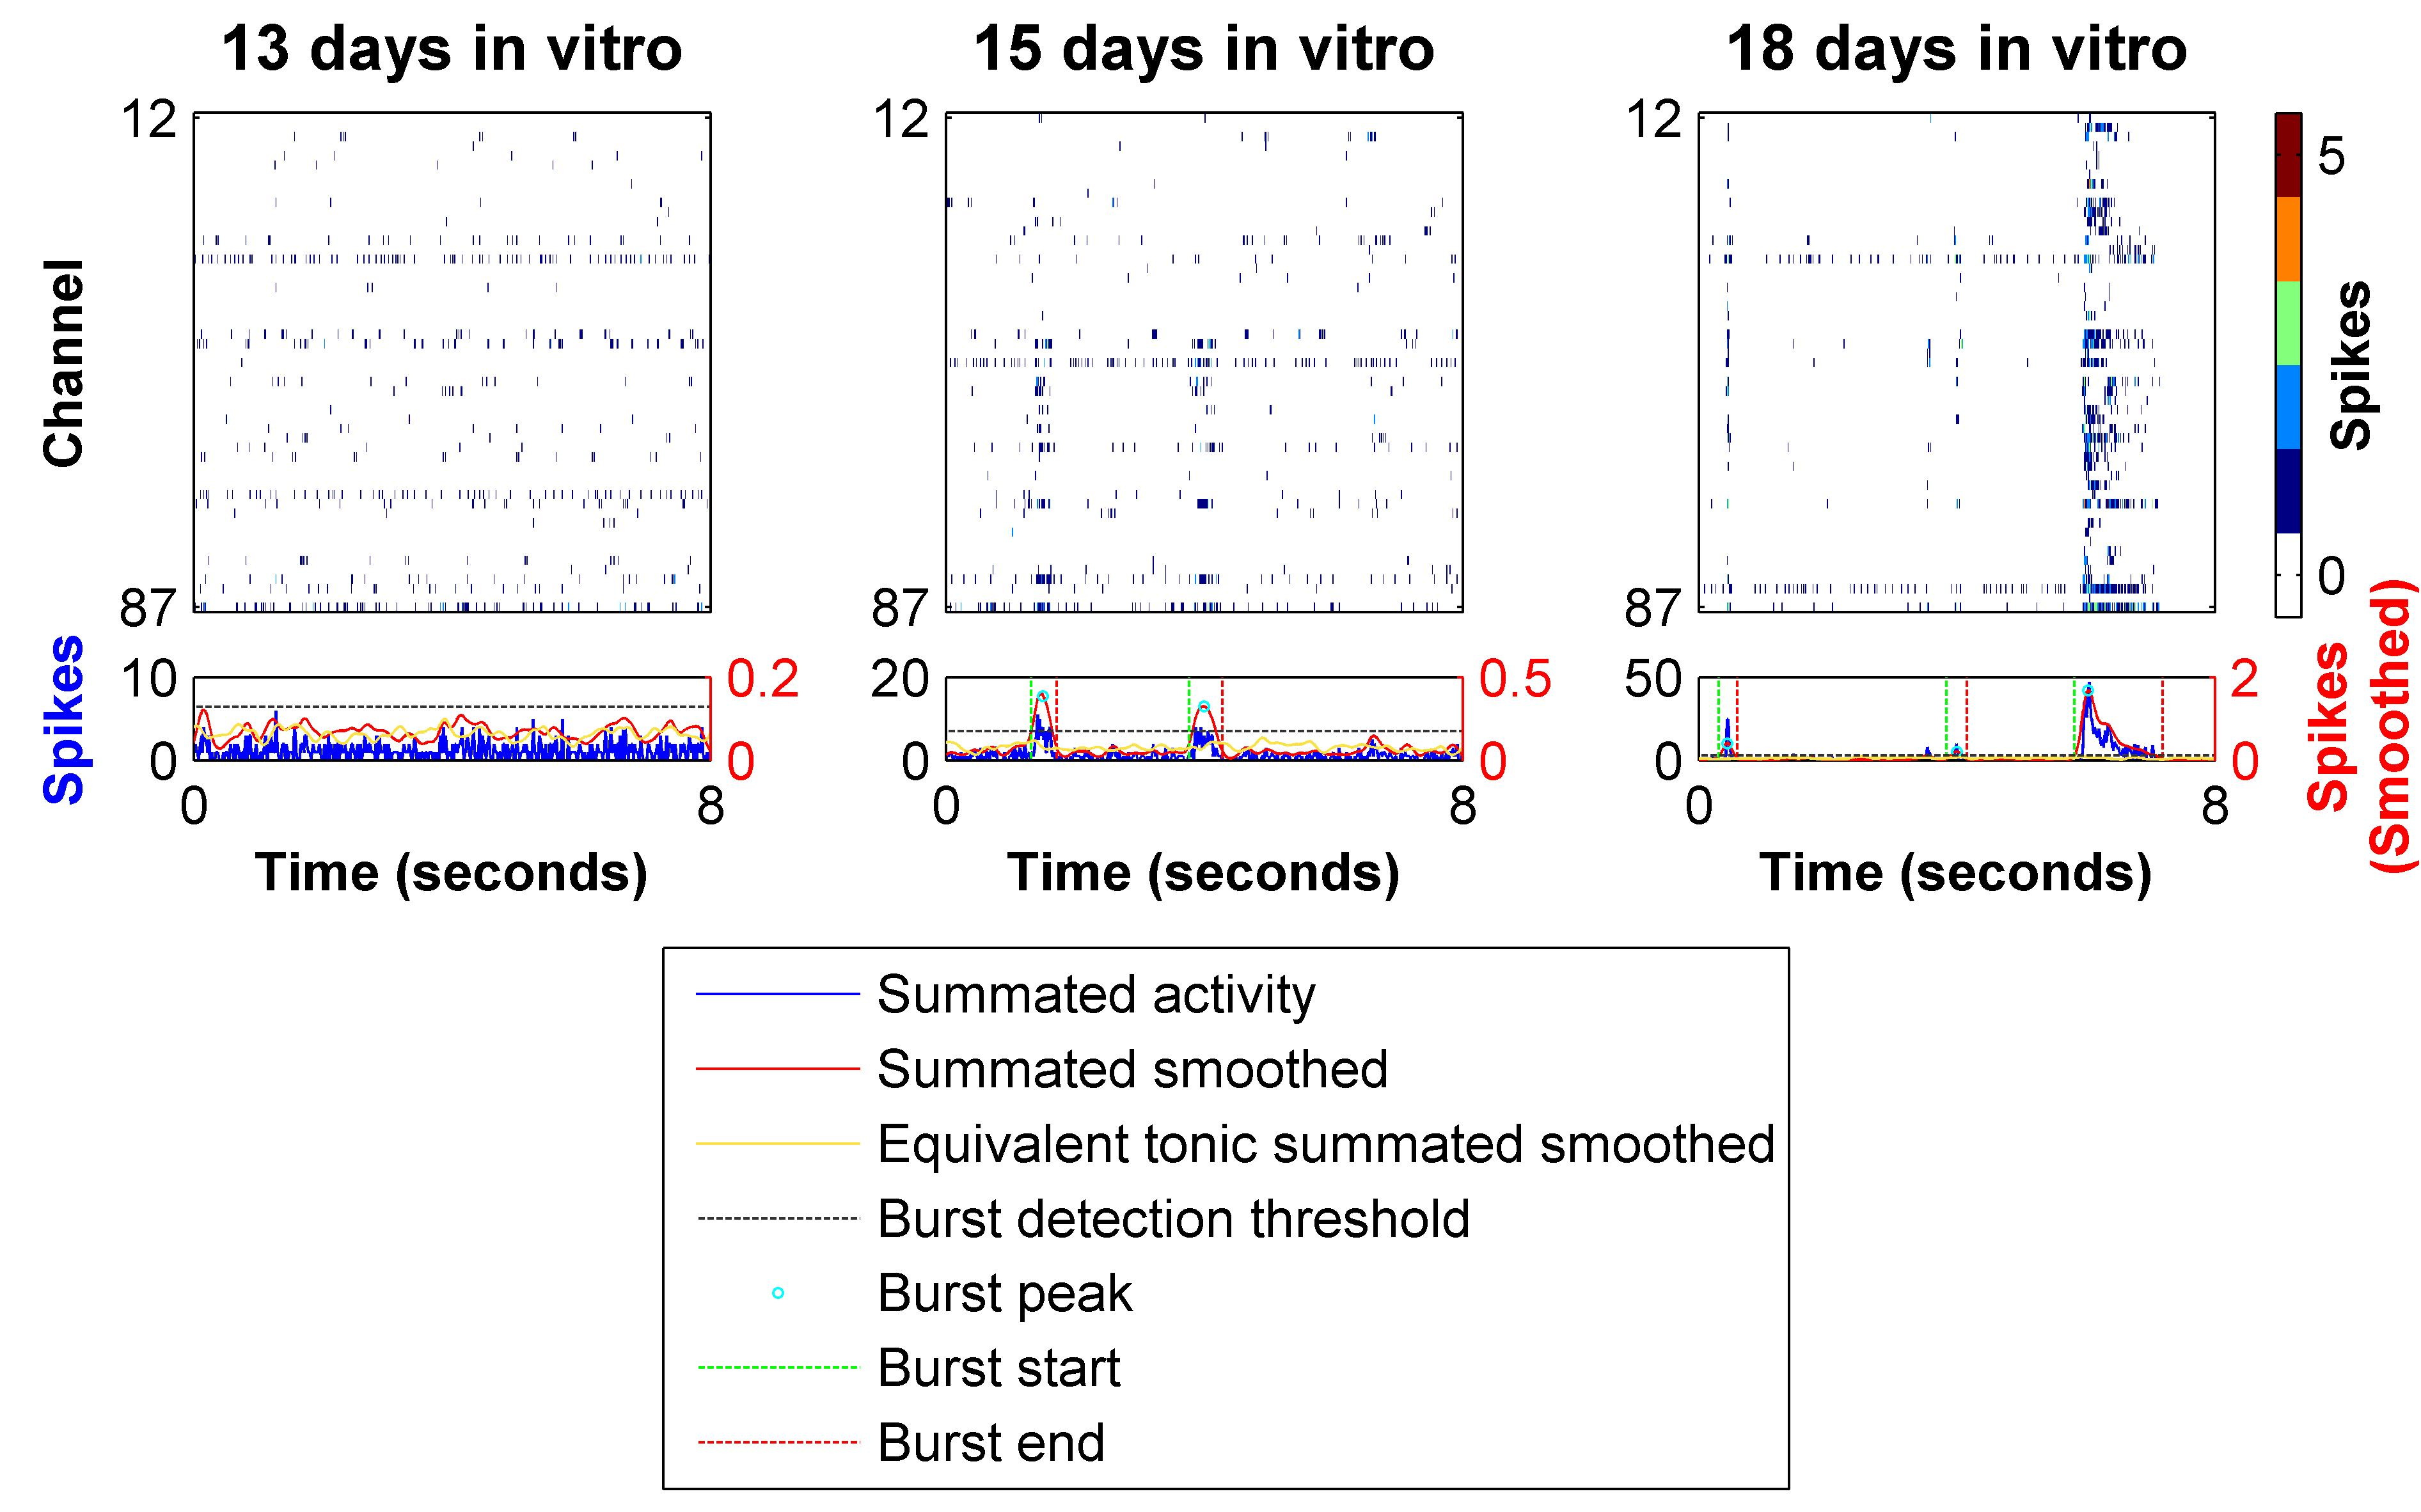
\includegraphics[width=15cm]{chapter2/figures/burstDetection/burstDetExample.jpg}
            \caption[Examples of burst detection output]{\textbf{The burst detection algorithm is sensitive to a range of synchronized burst scales.} Raster plots and their sum from a single cortical mouse culture at different developmental stages are shown. Also shown are derived curves used for the burst detection procedure and the outputs of the algorithm (i.e., burst peak, start and end points). See text for further details.}
            \label{fig:methods:burstDet}
          \end{figure}

\subsection{Functional connectivity analysis}
Computation of the functional connectivity (FC) measure completely followed the concepts introduced in \cite{le2007conditional} and where the ideas are explained in greater detail. Functional connectivity is defined between pairs of channels. The computation was performed directly on the channel raster plots at \(1ms\) binning without any smoothing and FC was essentially defined as the cross correlation between the plots normalized to the number of spikes in the first channel: \[FC_{i,j}[\tau]=\frac{\sum{t}^{}X_i[t]\cdot X_j[t-\tau]}{N_i},\] where \(X_i\), \(X_j\) are the channel raster plots, \(N_i\) is the number of spikes in channel \(i\) and the computation was performed for \(0\le \tau \le 500ms\). Thus the FC measure reflects the probability of observing a spike in channel \(j\) at time \(\tau\) given an occurrence of a spike in channel \(i\) at time \(0ms\). When the FC curve is not flat (i.e., it contains a peak) this indicates a true association between the channels. To characterize the FC curve it was further fitted to the following function, which essentially describes a hump of height \(M\) at a distance \(T\) from the y-axis with a baseline as offset \(o\) from the abscissa: \[FC_{fit}[\tau]=\frac{M}{1+\left(\frac{\tau-T}{w}\right)^{2}}+o.\]
A functional connection was considered to be present if, in the above fit, \(M>5\cdot o\), which indicates a significant peak. The fit also had to be rejected if it resulted in parameters with extreme values and so additional conditions were imposed: \(10<w<250\) and \(T<250\). FC was calculated only when both channels had at least 200 spikes as otherwise the generated curve was too noisy to analyze meaningfully.

Figure \ref{fig:methods:FC} shows example of functional connectivity curves and their respective fits to demonstrate that this measure was applied to our data with meaningful results.

We would like to emphasize that the parameter \(M\) above reflects the strength of the connection (i.e., the probability of observing paired spikes in the analyzed channels) and \(T\) is the characteristic time delay between such spikes. In this Ph.D work, we used two types of preparations, macrocultures and microcultures. In the case of macrocultures, the recordings sites were spread over a significantly larger area of tissue and this difference was indeed reflected in the values obtained for the parameter \(T\). In the case of macrocultures, values in the range of \(0-106ms\) were observed and 60\% of the values were smaller than \(1ms\). In the case of microcultures, a smaller range of \(0-20ms\) was observed and 96\%(!) of the values were smaller than \(1 ms\). These differences might reflect simply the proximity electrode pairs in the microculture recordings but it might also indicate a higher degree of coupling between the neurons in such preparations.

\begin{figure}[h]
\centering
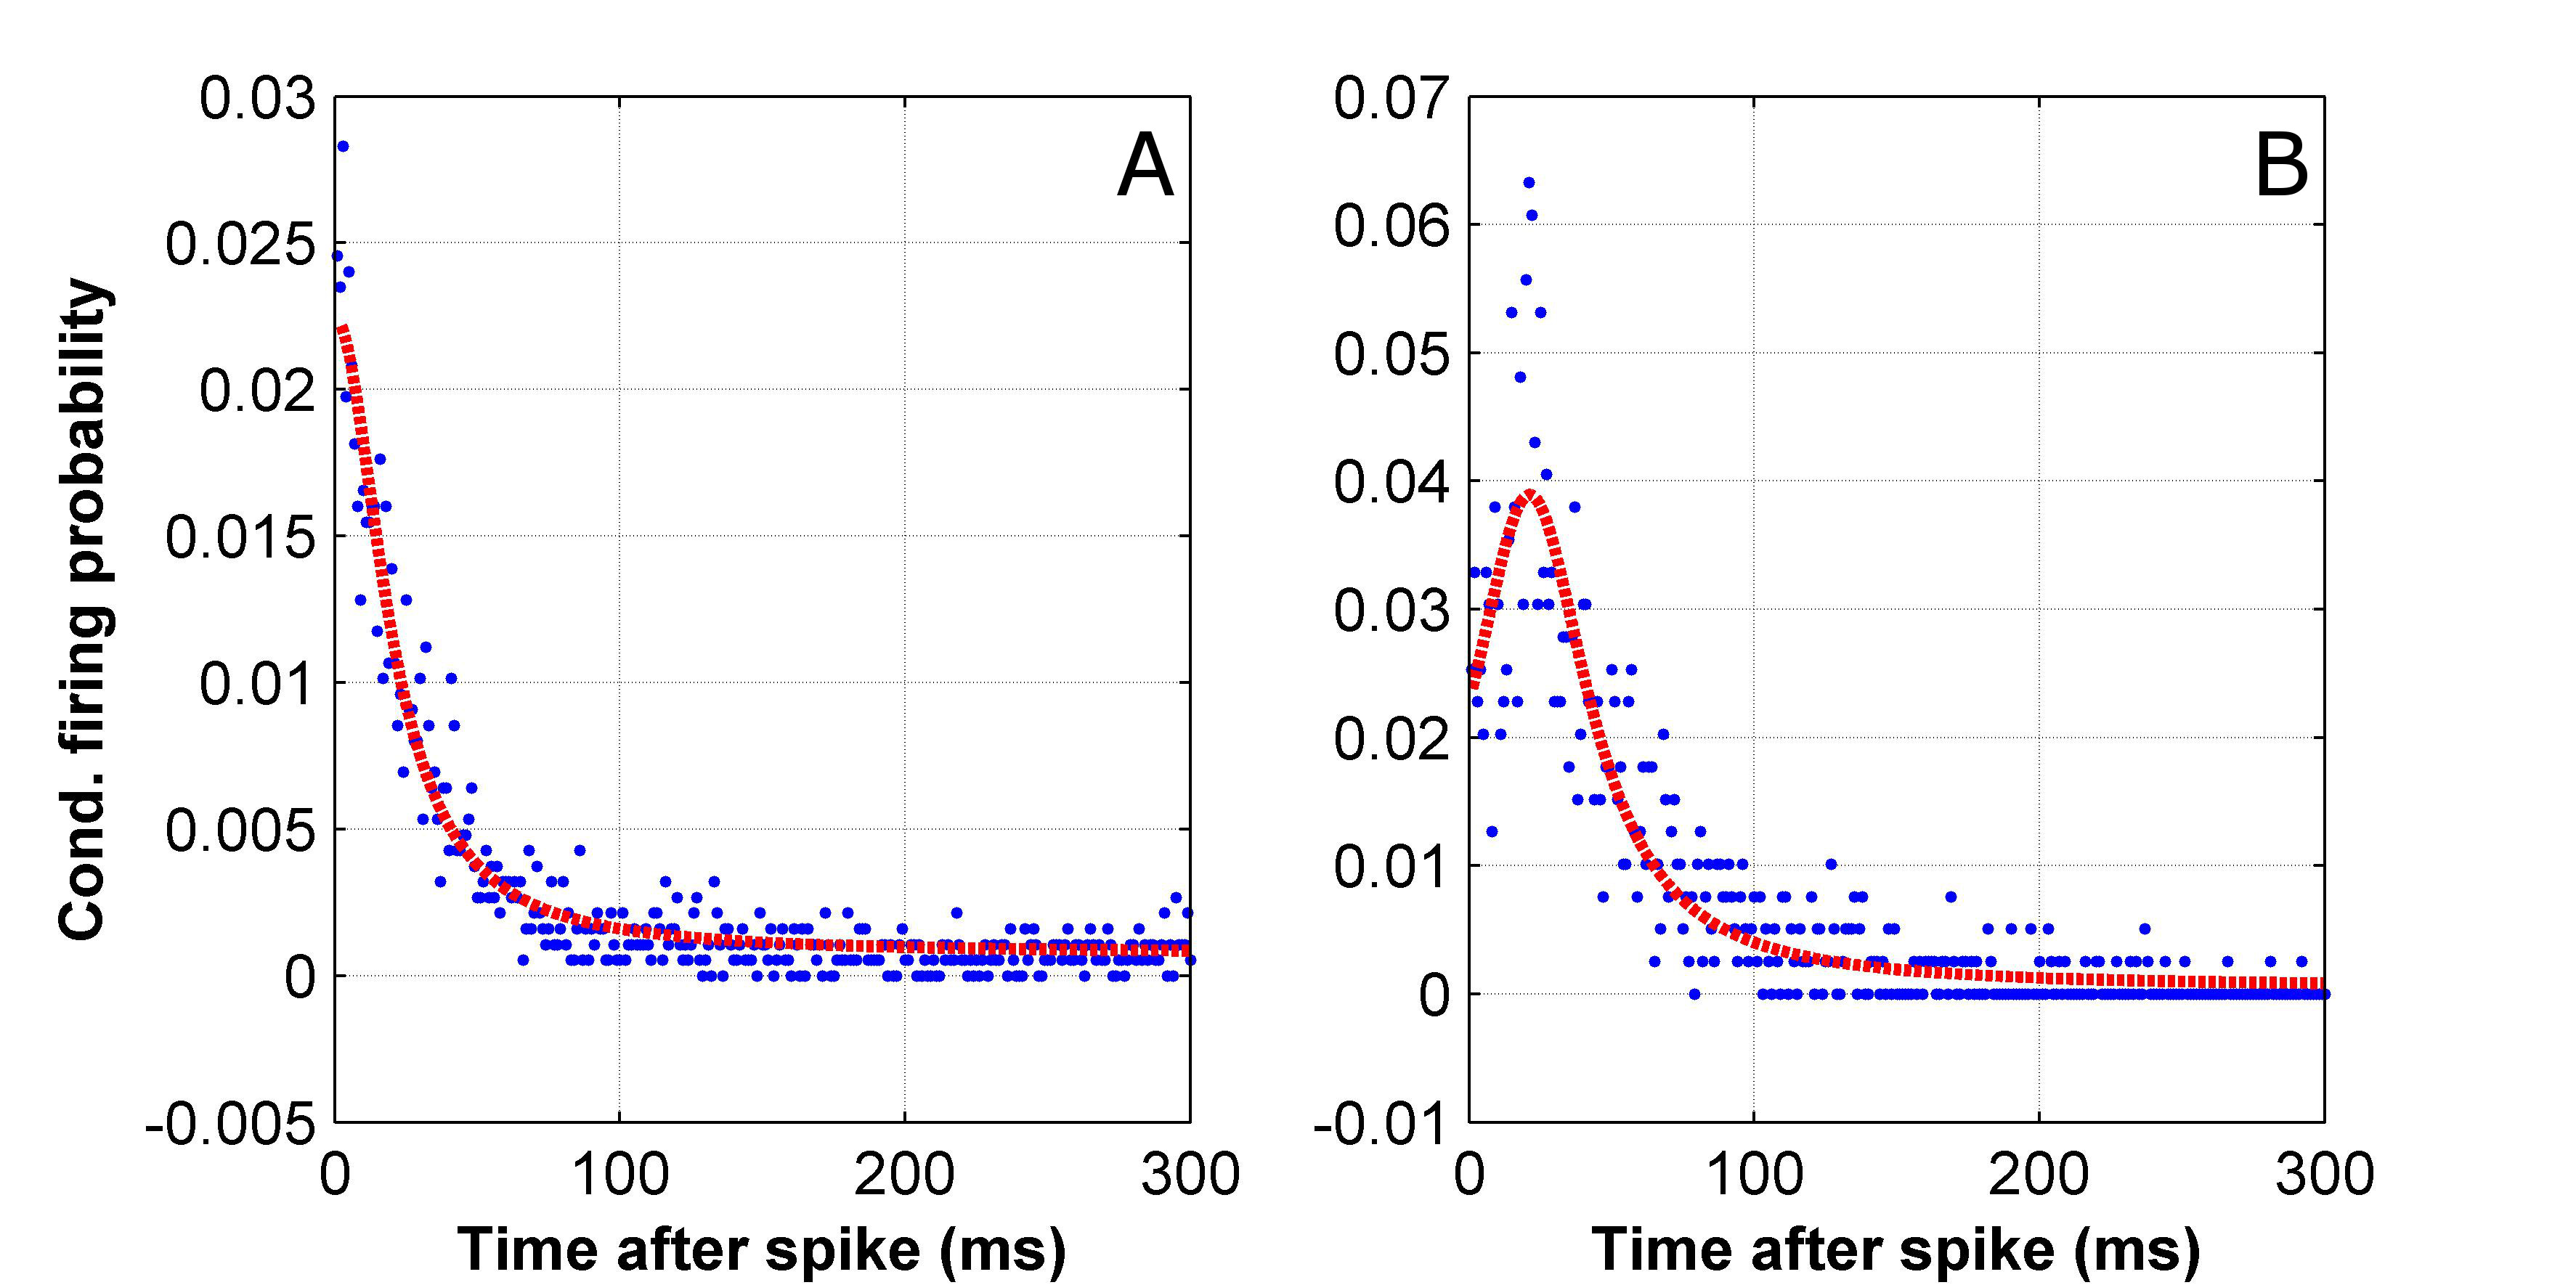
\includegraphics[width=15cm]{chapter2/figures/FCDemonstration/FCDemonstration.jpg}
\caption[Examples of functional connectivity curves]{\textbf{Functional connectivity curves exhibit localized peaks that reflect the coupling between neurons recorded at the analyzed pair of electrodes.} 2 FC curves are shown from a spontaneous activity recording in a mouse culture grown on a standard \(8\times 8\) MEA. (A) A FC curve with a peak at \(\approx 0ms\) (\(T=10\times 10^{-5}ms\)). This type of functional connection might represent a neuron pair that is strongly coupled or where both neurons are driven by similar synaptic input. (B) A FC curve with \(T=21ms\). This functional connection represents a characteristic propagation delay in the network.}

\label{fig:methods:FC}
\end{figure}
\label{sec:methods:FC}

\section{Conditioned media production}
In section \ref{sec:devices:viabilityAssay} we explored the link between the culture's viability under flow and the conditioning levels of the flow media. This required a standardized conditioning scale. Here we describe the production of such conditioned media and the definition of the standardized scale. Cortical cells were used for the purpose of media conditioning as they are available at larger quantities. These were seeded into T-12 flasks, \(3\times 10^6\) cells per flask, in a final volume of \(5 ml\). Flasks were kept in the incubator without changing the media until reaching the desired conditioning level at which point the media was collected and used for flow experiments. Conditioning level was calculated by: \(round\left(\frac{12\cdot DIV}{35}\right)\) where \(DIV\) is the number of days from plating. According to this scale, for every \(\approx\) 3 days in the flasks, the media accumulates 1 conditioning unit.
    \label{sec:methods:cond}



\section{Flow experiments}
\label{sec:methods:flow}
Flow control was performed with a pressure-driven microfluidics flow control system (Eleveflow, France) comprising a 4-channel pressure controller (\(0-200 mbar\) gauge pressure range, Elveflow, OBI) and 4 matching thermal mass flow sensors (\(0-7 \frac{\mu l}{min}\) sensing range, Elveflow, MFS2). The apparatus was controlled with the Elveflow software interface (SI2.6.1). The organization of this modern flow control system is illustrated in figure \ref{fig:methods:schematics}. The pressure controller uses fast piezoelectric valves to introduce or vent gas from reservoirs holding the flow media. This control method supports rapid pressure changes with a response time in the order of \(80ms\). We used a 5\% CO\textsubscript{2}/air gas supply to the pressure controller to keep the media CO\textsubscript{2} saturated. The pressure drives the media out of the reservoirs through tubing which are inline with the flow sensors. A PID control loop implemented in software utilizes the flow sensor data to control the flow rates. The flow PID parameters are accessible through the software and were used to control the flow responsiveness.

       \begin{figure}[!htb]
            \centering
            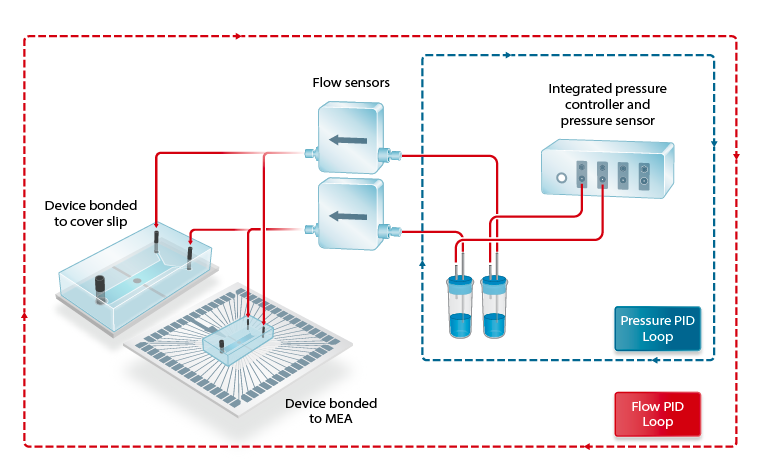
\includegraphics[width=14cm]{chapter2/figures/Schematics/schematics.png}
            \caption[Illustration of flow system]{\textbf{Illustration of flow system.} Pressure in media reservoirs is directly controlled to induce flow which is monitored via inline flow sensors. The control in the system is implemented via nested PID. The user defines the set value of the flow PID which utilizes the set value of the pressure PID.}
            \label{fig:methods:schematics}

        \end{figure}


We used polyether ether ketone (PEEK) tubing (\(360 \mu m\) OD \(150-250 \mu m\) ID, VICI, TPK.106, JR-T-5608-M3 or JR-T-5610-M3)
for the flow lines directly connected to the reservoirs. PEEK was selected on the basis of its low gas permeability and was expected to retain the CO\textsubscript{2} saturation of the media as it flows out of the reservoirs. The PEEK tubing entered a custom made environmental chamber heated to \(37\degree C\) with a 5\% CO\textsuperscript{2} atmosphere (figure \ref{fig:app:chamber}) through a small side hole. Inside the chamber, the PEEK lines were extended by flexible PTFE tubing with a larger ID of \(500\mu m\) which finally plugged into the device via a stainless steel \(1/32''\) needle. All PTFE lines inside the environmental chamber contained inline bubble traps which essentially comprised a PDMS block with a large internal cavity. Air arriving into the bubble trap cavity tended to float up to the upper PDMS surface and did not proceed with the flow. The location of the bubble traps along the flow line was as proximal as possible to the device inlets to minimize the chance of air bubbles forming in the intermediate flow line section. The total tubing volume inside the environmental chamber was 3 times larger than outside. This was purposefully designed to allow the media to reabsorb any CO\textsuperscript{2} lost during the travel in the ambient air from the reservoir to the chamber and heat up to \(37\degree C\). Each flow experiment was initiated by flushing the system with IPA, DDW and finally with the flow media. To connect a flow line to a device port its flow rate was set to \(1\frac{\mu l}{min}\) and it was plugged in only after an obvious drop was formed at the tip of the connector needle to assure that no air was introduced during the connection process. The inlets were always connected prior to the outlet because the latter flow line was loaded with fresh media which should not be allowed to reach the cells. The elasticity of the PDMS was normally enough to create a seal around the connector needle to prevent leaks. However, it should be noted that such leaks from the ports were the most common type experiment failure. Such leaks from the ports or due to failure of the PDMS-surface bond were detected by monitoring the flow rate in the outlet channel to assure that all the flow in the inlets is accounted for (i.e., outlet flow rate is sum of inlet rates).

In cases where flow experiments were performed on coverslip based devices (relevant for section \ref{sec:devices:viabilityAssay}) up to 3 devices could be placed under flow simultaneously using separate flow channels (figure \ref{fig:app:3Devices}). Outlets were combined into a single flow line using a PDMS junction or a ring connector. In the case of flow experiments that utilized self media (chapters \ref{chap:activityAndFlow} and \ref{chap:microculturePulses}) the sample had to be drained of its immersion media so as to transfer it to the flow system's media reservoirs. This was performed after the sample had been placed in the environmental chamber. In this case the sample had to be left with a drop of self media on top to prevent dehydration. After all the device ports were connected (2 or 3) the flow rates could were either set to a steady value (i.e., in the case of the steady flow experiments in chapters \ref{chap:devicesAndFlow} and \ref{chap:activityAndFlow}) or a more complex flow sequence was initiated (chapter \ref{chap:microculturePulses}). Pulsing experiments were controlled by a custom made Labview program which allowed personalized design of chemical and electrical stimulation sequences and communicated with the flow controller and the stimulator (see section \ref{sec:methods:stim}) via TTL pulses.






 \subsection{Viability analysis}
 To quantify the viability of the cultures under flow (section \ref{sec:devices:viabilityAssay}) the flow media was supplemented with \(2.5\frac{\mu g}{ml}\) Propidium Iodide. Dead cells leave behind exposed particles of condensed DNA appearing as fluorescent dots under Propidium Iodide staining. Consecutive fluorescent images of the same culture region in the device were taken every 1-2 hours. Bright field image of same region was also taken at the beginning of the flow session. Images were taken with a CCD camera (QuantEM 512SC, Photometrics or Grasshopper 2, PointGrey) mounted on a wide field fluorescence microscope (Brunel SP-99) and a TRITC ET filter set (Chroma). The number of dead cells in each image was counted automatically using ImageJ by thresholding the fluorescence image and counting the number of separate particles. The number of live cells was counted manually from inspection of the bright field image.
The proportion of live cells in each image was finally calculated as: \[\text{Proportion live cells} (i)=\frac{live(1)-(dead(i)-dead(1))}{live(1)},\] where \(live(1)\) is the number of live cells in initial bright field image and \(dead(i)\) is the dead cell count in image \(i\) of the time lapse.

 \begin{figure}[h]
     \centering
     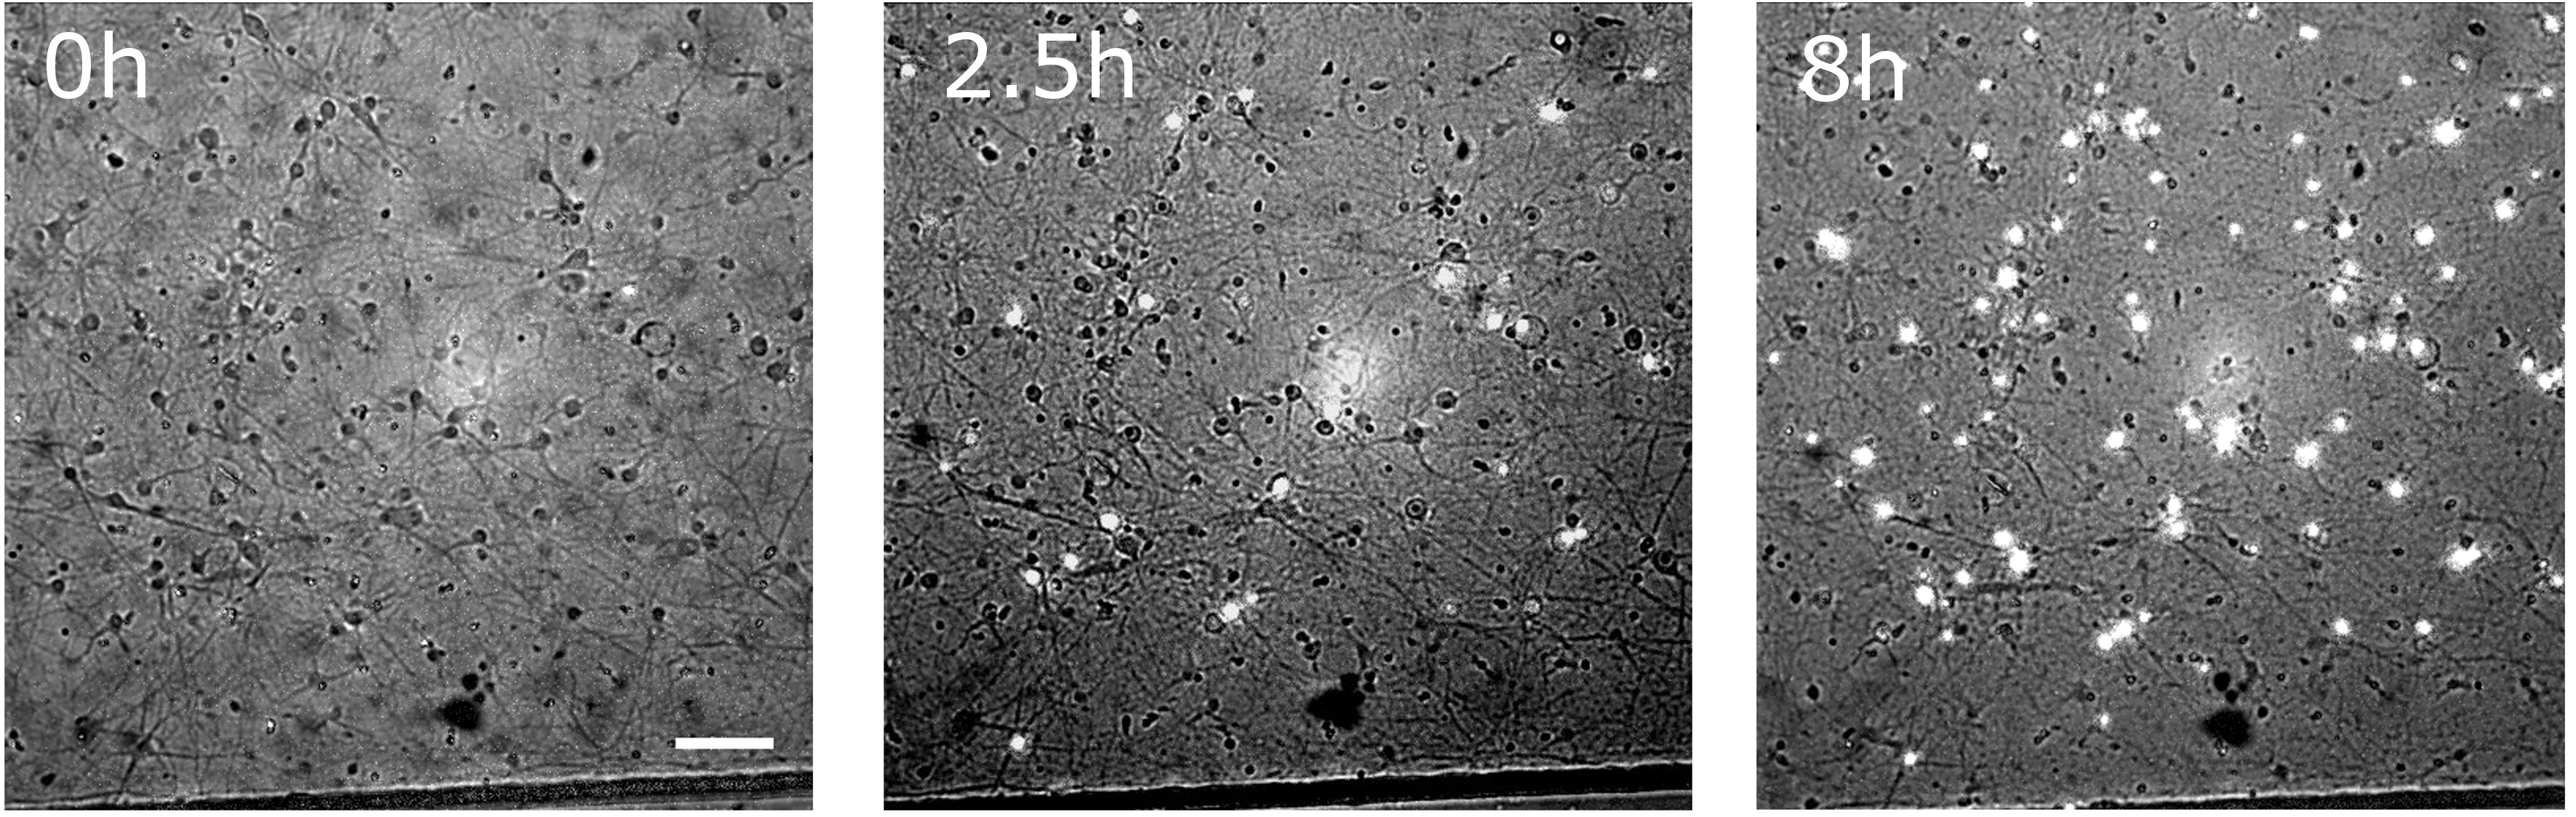
\includegraphics[width=15cm]{chapter2/figures/PIAssayIllustration/PIAssay.jpg}
     \caption[Example fluorescence images of Propidium Iodide staining under flow]{\textbf{Dead cells appear as fluorescent dots under flow with Propidium Iodide supplemented media.} Overlays of fluorescent (TRITC filter set) and bright field images of hippocampal cultures under flow with Propidium Iodide supplemented media. Fluorescent dots were automatically counted using ImageJ.}
     \label{fig:methods:PIAssay}

 \end{figure}

 \section{Immunofluorescence}
Device samples were washed in a phosphate buffered solution (PBS) by applying a drop on top and pulling through with a \(1ml\) syringe. This protocol was applied specifically in relatively deep microwell devices (\(120\mu m\), section \ref{sec:pulses:microcultures}). The shear protection conferred by these deep microwells prevented the microcultures from being washed away despite the relatively aggressive washing method. All consecutive washing steps in this protocol were applied in the same manner. The sample was fixated with a 4\% paraformaldehyde solution in PBS which also contained 4\% sucrose, \(20mM\) NaOH and \(5mM\) MgCl and pH corrected to 7.4. Next they were washed \(3\times\) with \(10mM\) Glycine in PBS and permeabilized by incubating in \(10mMm\) Glycine and 0.1\% Triton in PBS for 30 minutes.  As a next step they were washed with 0.1\% Triton in PBS and finally blocked through incubation in 3\% BSA for 1 hour. After the blocking, They were  incubated in primary antibodies (see below, 1:250 dilution) and 3\% BSA in PBS overnight at \(4\degree C\). The next day, the samples were washed \(3\times\) with 0.1\% Triton in PBS and incubated in secondary antibodies (see below, 1:500 dilution) and 3\% BSA in PBS. Finally, samples were washed again \(3\times\) in 0.1\% Triton in PBS and incubated in \(0.01 \frac{\mu g}{ml}\) DAPI in PBS for 5 minutes following which they were washed in PBS and imaged using a fluorescent microscope (Nikkon Eclipse Ti) and an EMCCD camera. To detect glial cells, goat anti-glial fibrillary acidic protein monoclonal antibody was used (GFAP, Abcam, ab53554). Neurons were detected using Rabbit Anti-\textbeta III-Tubulin, (Abcam, ab78078). The corresponding secondary antibodies were Alexa Fluor 647 chicken anti-goat (Life Technologies, A21469, imaged with CY5 filter set by Chroma) and Alexa fluor 488 donkey anti-rabit (Life Technologies, A21206, imaged with FITC filter set by Chroma).



